% 第 10 章 高级领域特定语言
\renewcommand{\codeInset}{63bp}
在上一章中，我们开发了一种领域特定语言（Domain-Specific Language，DSL）。本章将从以下几个方面改进这门语言：

我们将添加选择和迭代。具体来说，我们将加入 \texttt{if} 和 \texttt{while} 指令。在上一章的语言中，动作是按顺序直接执行的；而在本章中，可以在多个分支之间做出选择，也可以对一部分代码进行迭代。

我们将添加变量。在上一章中，一个名字只能被赋值一次；而在本章中，赋给名字的值可以在程序执行过程中被重新赋值。

我们将添加带有参数和返回值的函数。在上一章中，程序由一连串指令组成；而在本章中，程序由一连串函数组成。与 C++ 一样，程序必须有一个 \texttt{main} 函数作为执行的起点。

最后，我们将在从源代码到查看器的处理流程中再增加一个模块。在上一章中，解析器生成一连串动作，由查看器显示；而在本章中，解析器生成一连串指示（directive），指示再由求值器求值为动作。

由于本章的语言支持选择、迭代、变量和函数调用，它已经开始像一门传统的编程语言了。

本章将涵盖以下主题：

\begin{itemize}
\item 与上一章一样，我们先通过一个示例非正式地查看 DSL 的源代码。不过，这个示例会用到变量和函数调用，还会用到 \texttt{if} 和 \texttt{while} 指令。
\item 然后，我们用文法（grammar）正式定义这门语言。文法是上一章文法的扩展，我们将加入函数定义、函数调用和函数返回的指令，以及选择（\texttt{if}）和迭代（\texttt{while}）。
\item 定义好文法之后，我们编写扫描器（scanner）。本章的扫描器与上一章几乎完全相同，唯一的区别是增加了几个关键字。
\item 写好扫描器之后，我们编写解析器（parser）。解析器是上一章解析器的扩展，我们为函数、选择和迭代添加了相应的方法。不过，上一章的解析器生成的是一连串动作，由查看器读取并执行；而本章的解析器生成的则是一连串指示，由求值器读取。
\item 本章接下来的环节是求值器（evaluator），而不是查看器。求值器接收解析器生成的指示序列，生成一连串动作，由查看器读取并执行。求值器使用为名字赋值的映射。其中有一个值映射栈（value map stack），确保每个被调用的函数都获得自己的全新值映射；还有一个值栈（value stack），在求值表达式时存放临时值；最后还有一个调用栈（call stack），存放函数调用的返回地址。
\item 最后，查看器的工作方式与上一章相同：它遍历求值器生成的动作列表，在 Qt 部件中显示图形对象。
\end{itemize}

\section{通过示例改进源语言}

我们来看一个新示例：定义并调用一个名为 \texttt{triangle} 的函数，用不同的画笔以不同的尺寸绘制三角形。注意，函数不必按任何特定顺序出现。

我们先把 \texttt{left} 和 \texttt{length} 变量设为 50，它们分别存放第一个三角形最左侧角的 x 坐标和底边长度。接着把 \texttt{index} 变量设为 0，它的值将用于 \texttt{while} 迭代：

\begin{codebox}
function main() {
  left = 50;
  length = 50;
  index = 0;
\end{codebox}

只要 \texttt{index} 小于 4，我们就继续迭代。注意，本章在 Value 类中加入了布尔值。当 \texttt{index} 为偶数时，我们把画笔样式设为实线；当 \texttt{index} 为奇数时，则把画笔样式设为虚线。注意，我们还用关系表达式和取模运算符（\texttt{\%}）扩展了这门语言：

\begin{codebox}
  while (index < 4) {
    if ((index % 2) == 0) {
      SetPenStyle(SolidLine);
    }
    else {
      SetPenStyle(DashLine);
    }
\end{codebox}

我们设置三角形的左上角点，并调用 \texttt{drawTriangle} 函数来实际绘制三角形：

\begin{codebox}
            topLeft = point(left, 25);
            call drawTriangle(topLeft, length);
\end{codebox}

调用 \texttt{triangle} 之后，我们增大下一个三角形的底边长度，并移动最左侧角的位置：

\begin{codebox}
    length = length + 25;
    left = left + length;
    index = index + 1;
  }
}
\end{codebox}

在 \texttt{drawTriangle} 函数中，我们调用 \texttt{getTopRight} 和 \texttt{getBottomMiddle} 函数来获得三角形的右上点和底边中点。最后，我们调用 \texttt{drawLine} 来绘制三角形的三条边：

\begin{codebox}
function drawTriangle(topLeft, length) {
  topRight = call getTopRight(topLeft, length);
  bottomMiddle = call getBottomMiddle(topLeft, length);
  drawLine(topLeft, topRight);
  drawLine(topRight, bottomMiddle);
\end{codebox}

\begin{codebox}
  drawLine(bottomMiddle, topLeft);
}
\end{codebox}

\texttt{getTopRight} 函数提取左上角点的 x 和 y 坐标，并返回一个 x 坐标增加了三角形底边长度的点：

\begin{codebox}
function getTopRight(topLeft, length) {
  return point(xCoordinate(topLeft) + length,
               yCoordinate(topLeft));
}
\end{codebox}

\texttt{getBottomMiddle} 函数同样提取左上角点的 x 和 y 坐标，然后计算出底边中点的 x 和 y 坐标并返回该点：

\begin{codebox}
function getBottomMiddle(topLeft, length) {
  left = xCoordinate(topLeft);
  top = yCoordinate(topLeft);
  middle = left + length / 2;
  bottom = top + length;
  return point(middle, bottom);
}
\end{codebox}

运行代码后，输出如下截图所示：

\begin{center}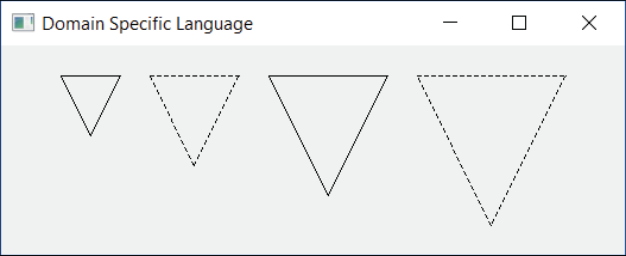
\includegraphics[width=0.5\textwidth]{images/p404_i08.png}\end{center}

\section{改进文法}

本章将改进我们这门语言的文法。首先，程序由一连串函数而非指令组成。严格来说，程序可以不含任何函数，但此时语义错误会报告缺少 \texttt{main} 函数：

\begin{codebox}
program -> functionDefinitionList
functionDefinitionList -> functionDefinition*
\end{codebox}

函数的定义由关键字 \texttt{function}、括号括起的一列名字以及花括号括起的一列指令组成。nameList 由零个或多个名字组成，名字之间用逗号分隔：

\begin{codebox}
functionDefinition -> function name(nameList) { instructionList }
\end{codebox}

在指令方面，我们加入了函数调用。我们既可以把函数作为一条指令直接调用（前面示例中的 call drawTriangle），也可以把它作为表达式的一部分来调用（call getTopRight 和 call getBottomMiddle）。

我们还加入了 \texttt{while} 指令以及 \texttt{if} 指令——后者可以带也可以不带 \texttt{else} 部分。最后还有块指令：由花括号括起的一列指令：

\begin{codebox}
instruction -> callExpression ;
             | while (expression) instruction
             | if (expression) instruction
             | if (expression) instruction else instruction
             | { instructionList }
             | ...
callInstruction -> callExpression ;
\end{codebox}

至于表达式，唯一的区别是我们加入了函数调用。expressionList 是一列由零个或多个表达式组成的列表，表达式之间用逗号分隔：

\begin{codebox}
primaryExpression -> call name(expressionList)
                   |
\end{codebox}

\section{Token 与扫描器}

与上一章一样，这门语言最终生成的目标代码仍是动作，只不过这次是由求值器而非解析器生成。Action 类与上一章的类完全相同，Value 类和 ViewerWidget 类以及颜色和错误处理也是如此。不过，Token 类和 Scanner 类做了扩展，TokenId 枚举增加了更多的词法单元（token）标识。

\medskip\noindent{\ttfamily\bfseries Token.h}

\begin{codebox}
class Token {
  // ...
  enum TokenId {BlockId, CallId, ElseId, FunctionId, GotoId,
                IfId, IfNotGotoId, ReturnId, WhileId, // ...
               };
  // ...
};
\end{codebox}

同样，Scanner 中的 init 也加入了这些关键字：

\medskip\noindent{\ttfamily\bfseries Scanner.cpp}

\begin{codebox}
void Scanner::init() {
  ADD_TO_KEYWORD_MAP(CallId)
  ADD_TO_KEYWORD_MAP(ElseId)
  ADD_TO_KEYWORD_MAP(FunctionId)
  ADD_TO_KEYWORD_MAP(IfId)
  ADD_TO_KEYWORD_MAP(ReturnId)
  ADD_TO_KEYWORD_MAP(WhileId)
// ...
}
\end{codebox}

\section{解析器}

解析器增加了与文法新规则相对应的方法。此外，本章的解析器不再生成动作，而是生成指示。原因在于：上一章的源代码中的指令是从头到尾顺序执行的，而本章的源代码包含选择、迭代和函数调用，它们会改变指令的执行流程。因此，引入一个中间层是合理的——解析器生成指示，指示再被求值为动作。

由于本章的语言支持函数，我们需要一个 Function 类来存放函数。它存放形式参数的名字和函数的起始地址。

\medskip\noindent{\ttfamily\bfseries Function.h}

\begin{codebox}
#ifndef FUNCTION_H
#define FUNCTION_H
#include <QtWidgets>
#include "Value.h"
#include "Action.h"
class Function {
  public:
    Function() {}
    Function(const QList<QString>& nameList, int address);
    const QList<QString>& nameList() const {return m_nameList;}
    int address() {return m_address;}
    Function(const Function& function);
    Function operator=(const Function& function);
  private:
    QList<QString> m_nameList;
    int m_address;
};
#endif // FUNCTION_H
\end{codebox}

Function.cpp 文件存放 Function 类方法的定义。

\medskip\noindent{\ttfamily\bfseries Function.cpp}

\begin{codebox}
#include "Function.h"
Function::Function(const QList<QString>& nameList, int address)
 :m_nameList(nameList),
  m_address(address) {
  // Empty.
}
Function::Function(const Function& function)
 :m_nameList(function.m_nameList),
  m_address(function.m_address) {
  // Empty.
}
Function Function::operator=(const Function& function) {
  m_nameList = function.m_nameList;
  m_address = function.m_address;
  return *this;
}
\end{codebox}

由于本章的解析器生成的是一连串指示而非动作，我们还需要一个 Directive 类来存放指示。大多数情况下，Directive 对象只存放 TokenId 枚举中的标识。不过，在函数调用的场合，我们需要存放函数名和实际参数的个数；在函数定义的场合，我们存放对 Function 对象的引用；在表达式由一个名字或一个值构成的场合，我们需要存放名字或值；最后还有几种跳转指示，此时我们需要存放地址。

\medskip\noindent{\ttfamily\bfseries Directive.h}

\begin{codebox}
#ifndef DIRECTIVE_H
#define DIRECTIVE_H
#include <QtWidgets>
#include "Token.h"
#include "Value.h"
#include "Function.h"
class Directive {
  public:
    Directive(TokenId tokenId);
    Directive(TokenId tokenId, int address);
    Directive(TokenId tokenId, const QString& name);
    Directive(TokenId tokenId, const QString& name,
              int parameters);
    Directive(TokenId tokenId, const Value& value);
    Directive(TokenId tokenId, const Function& function);
    Directive(const Directive& directive);
    Directive operator=(const Directive& directive);
    TokenId directiveId() {return m_directiveId;}
    const QString& name() {return m_name;}
    const Value& value() {return m_value;}
    const Function& function() {return m_function;}
    int parameters() const {return m_parameters;}
    int address() const {return m_address;}
    void setAddress(int address) {m_address = address;}
  private:
    TokenId m_directiveId;
    QString m_name;
    int m_parameters, m_address;
    Value m_value;
    Function m_function;
};
#endif // DIRECTIVE_H
\end{codebox}

Directive.cpp 文件存放 Directive 类方法的定义。

\medskip\noindent{\ttfamily\bfseries Directive.cpp}

\begin{codebox}
#include "Directive.h"
\end{codebox}

大多数情况下，我们只创建一个带有指示标识的 Directive 对象：

\begin{codebox}
Directive::Directive(TokenId directiveId)
 :m_directiveId(directiveId) {
  // Empty.
}
\end{codebox}

跳转指示需要跳转地址：

\begin{codebox}
Directive::Directive(TokenId directiveId, int address)
 :m_directiveId(directiveId),
  m_address(address) {
  // Empty.
}
\end{codebox}

给变量赋值时，我们需要变量的名字；不过不需要值，因为值将存放在栈上。另外，当表达式由一个名字构成时，我们需要存放这个名字：

\begin{codebox}
Directive::Directive(TokenId directiveId, const QString& name)
 :m_directiveId(directiveId),
  m_name(name) {
  // Empty.
}
\end{codebox}

函数调用的指示需要函数名和实际参数的个数：

\begin{codebox}
Directive::Directive(TokenId directiveId, const QString& name,
                     int parameters)
 :m_directiveId(directiveId),
  m_name(name),
  m_parameters(parameters) {
  // Empty.
}
\end{codebox}

当表达式仅由一个值构成时，我们直接把值存放在指示中：

\begin{codebox}
Directive::Directive(TokenId directiveId, const Value& value)
 :m_directiveId(directiveId),
  m_value(value) {
  // Empty.
}
\end{codebox}

最后，在函数定义中我们存放一个 Function 类的对象：

\begin{codebox}
Directive::Directive(TokenId directiveId,
                     const Function& function)
 :m_directiveId(directiveId),
  m_function(function) {
  // Empty.
}
\end{codebox}

Parser 类增加了与文法新规则相对应的方法：函数定义以及 \texttt{if}、\texttt{while}、\texttt{call} 和 \texttt{return} 指令。

\medskip\noindent{\ttfamily\bfseries Parser.h}

\begin{codebox}
// ...
class Parser {
  private:
    void functionDefinitionList();
    void functionDefinition();
\end{codebox}

nameList 方法收集函数的形式参数，而 expressionList 收集函数调用的实际参数：

\begin{codebox}
            QList<QString> nameList();
            int expressionList();
\end{codebox}

Parser 类中还加入了 callExpression 方法，因为函数既可以作为一条指令被显式调用，也可以作为表达式的一部分被调用：

\begin{codebox}
    void callExpression();
    // ...
};
\end{codebox}

Parser.cpp 文件存放 Parser 类方法的定义。本章解析器的起始方法是 functionDefinitionList，它不断调用 functionDefinition，直到到达文件末尾为止。

\medskip\noindent{\ttfamily\bfseries Parser.cpp}

\begin{codebox}
void Parser::functionDefinitionList() {
  while (m_lookAHead.id() != EndOfFileId) {
    functionDefinition();
  }
}
\end{codebox}

functionDefinition 方法解析一个函数定义。我们先匹配 \texttt{function} 关键字，并把函数名存放起来：

\begin{codebox}
void Parser::functionDefinition() {
  match(FunctionId);
  QString name = m_lookAHead.name();
  match(NameId);
\end{codebox}

函数名后面是括号括起的参数名字列表。我们把名字列表存放在 nList 字段中。不能把这个字段命名为 nameList，因为这个名字已经被同名方法占用了：

\begin{codebox}
  match(LeftParenthesisId);
  QList<QString> nList = nameList();
  match(RightParenthesisId);
\end{codebox}

我们把指示列表的当前大小存为函数的起始地址，用名字列表和起始地址创建一个 Function 对象，并把带有该函数的 Directive 对象加入指示列表：

\begin{codebox}
   int startAddress = (int) m_directiveList.size();
   Function function(nList, startAddress);
   m_directiveList.push_back(Directive(FunctionId, function));
\end{codebox}

名字列表后面是由花括号括起的一列指令：

\begin{codebox}
  match(LeftBracketId);
  instructionList();
  match(RightBracketId);
\end{codebox}

为了确保函数确实把控制权交还给调用它的函数，我们加入一个带有 \texttt{return} 词法单元标识的 Directive 对象：

\begin{codebox}
  m_directiveList.push_back(Directive(ReturnId));
\end{codebox}

函数定义完毕后，我们检查没有其他同名函数：

\begin{codebox}
  check(!m_functionMap.contains(name),
        "function "" + name + "" already defined");
\end{codebox}

如果函数名为 \texttt{main}，它就是程序的起始函数，不能带有参数：

\begin{codebox}
  check(!((name == "main") && (nList.size() > 0)),
        "function "main" cannot have parameters");
\end{codebox}

最后，我们把函数加入 functionMap：

\begin{codebox}
  m_functionMap[name] = function;
}
\end{codebox}

nameList 方法解析括号内以逗号分隔的名字列表：

\begin{codebox}
QList<QString> Parser::nameList() {
  QList <QString> nameList;
\end{codebox}

只要没有遇到右括号，我们就继续：

\begin{codebox}
  while (m_lookAHead.id() != RightParenthesisId) {
    QString name = m_lookAHead.name();
    nameList.push_back(name);
    match(NameId);
\end{codebox}

匹配完名字后，我们检查下一个词法单元是否为右括号。如果是，说明已到达名字列表末尾，我们便中断迭代：

\begin{codebox}
    if (m_lookAHead.id() == RightParenthesisId) {
      break;
    }
\end{codebox}

如果下一个词法单元不是右括号，我们就假定它是逗号，匹配它，然后继续迭代处理下一个表达式：

\begin{codebox}
    match(CommaId);
  }
\end{codebox}

最后，在返回名字列表之前，我们需要检查列表中没有名字出现两次。我们遍历名字列表，把名字加入一个集合：

\begin{codebox}
  QSet<QString> nameSet;
  for (const QString& name : nameList) {
    if (nameSet.contains(name)) {
      semanticError("parameter "" + name + "" defined twice");
    }
    nameSet.insert(name);
  }
  return nameList;
}
\end{codebox}

本章的 instructionList 方法看起来略有不同，因为它位于一个指令块内部。只要没有遇到右花括号，我们就继续迭代：

\begin{codebox}
void Parser::instructionList() {
  while (m_lookAHead.id() != RightBracketId) {
    instruction();
  }
}
\end{codebox}

由于函数既可以作为指令被显式调用，也可以作为表达式的一部分，因此在调用指令的场合，我们只需调用 callExpression 并匹配分号：

\begin{codebox}
void Parser::instruction() {
  switch (m_lookAHead.id()) {
    case CallId:
      callExpression();
      match(SemicolonId);
      break;
\end{codebox}

在 \texttt{return} 指令中，我们匹配 \texttt{return} 关键字，并检查其后是否跟着分号。如果没有跟着分号，我们就解析一个表达式，然后假定下一个词法单元是分号。注意，我们不存放表达式的结果，求值器稍后会把这个值放到栈上：

\begin{codebox}
    case ReturnId:
      match(ReturnId);
      if (m_lookAHead.id() != SemicolonId) {
        expression();
      }
      m_directiveList.push_back(Directive(ReturnId));
      match(SemicolonId);
      break;
\end{codebox}

对于 \texttt{if} 关键字，我们匹配它并解析一个由括号括起的表达式：

\begin{codebox}
    case IfId: {
        match(IfId);
        match(LeftParenthesisId);
        expression();
        match(RightParenthesisId);
\end{codebox}

如果表达式求值为假，我们就要跳过 \texttt{if} 表达式后面的那条指令。因此，我们加入一条 IfNotGoto 指示，打算跳过 \texttt{if} 关键字后面的指令：

\begin{codebox}
        int ifNotIndex = (int) m_directiveList.size();
        m_directiveList.push_back(Directive(IfNotGotoId, 0));
        instruction();
\end{codebox}

如果这条指令后面跟着 \texttt{else} 关键字，我们就匹配它，并加入一条 Goto 指示——当 \texttt{if} 指令的表达式为真时，打算跳过 \texttt{else} 部分：

\begin{codebox}
        if (m_lookAHead.id() == ElseId) {
          match(ElseId);
          int elseIndex = (int) m_directiveList.size();
          m_directiveList.push_back(Directive(GotoId, 0));
\end{codebox}

然后我们设置前面那条 IfNotGoto 指示的跳转地址。如果表达式不为真，程序就应跳到这一点：

\begin{codebox}
          m_directiveList[ifNotIndex].
            setAddress((int) m_directiveList.size());
          instruction();
\end{codebox}

另一方面，如果 \texttt{if} 指令的表达式为真，程序就应跳过 \texttt{else} 部分到达这一点：

\begin{codebox}
          m_directiveList[elseIndex].
            setAddress((int) m_directiveList.size());
        }
\end{codebox}

如果 \texttt{if} 指令后面没有跟 \texttt{else} 关键字，那么当表达式不为真时，程序就应跳到程序中的这一点：

\begin{codebox}
        else {
          m_directiveList[ifNotIndex].
            setAddress((int) m_directiveList.size());
        }
      }
      break;
\end{codebox}

对于 \texttt{while} 关键字，我们匹配它，并把指示列表的当前下标存放起来，以便程序在每次迭代之后都能跳回这一点：

\begin{codebox}
    case WhileId: {
        match(WhileId);
        int whileIndex = (int) m_directiveList.size();
\end{codebox}

然后我们解析表达式及其两侧的括号：

\begin{codebox}
        match(LeftParenthesisId);
        expression();
        match(RightParenthesisId);
\end{codebox}

当表达式不为真时，我们加入一条 IfNotGoto 指示，让程序跳出迭代：

\begin{codebox}
        int ifNotIndex = (int) m_directiveList.size();
        m_directiveList.push_back(Directive(IfNotGotoId, 0));
        instruction();
\end{codebox}

我们在 \texttt{while} 表达式后面的那条指令之后加入一条 Goto 指示，让程序在每次迭代结束时都能跳回表达式处：

\begin{codebox}
        m_directiveList.push_back(Directive(GotoId, whileIndex));
\end{codebox}

最后，我们把 \texttt{while} 指令开头的 IfNotGoto 指示的地址设置好，这样当表达式不为真时，它就能跳到程序中的这一点：

\begin{codebox}
        m_directiveList[ifNotIndex].
          setAddress((int) m_directiveList.size());
      }
      break;
\end{codebox}

遇到左花括号时，我们面对的是由花括号括起的一串指令。我们解析这一对花括号，并调用 instructionList：

\begin{codebox}
    case LeftBracketId:
      match(LeftBracketId);
      instructionList();
      match(RightBracketId);
      break;
\end{codebox}

最后，遇到名字时，我们面对的是一条赋值。我们匹配名字词法单元和赋值运算符（\texttt{=}），解析表达式，然后匹配分号。接着，我们向指示列表加入一个 Assign 对象，其中存放着将要被赋值的名字。注意，我们不存放表达式的值，因为求值器稍后会把它压入值栈：

\begin{codebox}
    case NameId: {
        QString name = m_lookAHead.name();
        match(NameId);
        match(AssignId);
        expression();
        match(SemicolonId);
        m_directiveList.push_back(Directive(AssignId, name));
      }
      break;
      // ...
  }
}
\end{codebox}

callExpression 方法匹配 \texttt{call} 关键字，存放函数名，解析参数表达式，并向指示列表加入一条携带该调用的 Directive 对象。注意，此时我们不检查函数是否存在，也不统计参数个数，因为函数可能尚未定义。所有类型检查都由后面的求值器负责完成：

\begin{codebox}
void Parser::callExpression() {
  match(CallId);
  QString name = m_lookAHead.name();
  match(NameId);
  match(LeftParenthesisId);
  int size = expressionList();
  match(RightParenthesisId);
  m_directiveList.push_back(Directive(CallId, name, size));
}
\end{codebox}

expressionList 方法解析一列表达式。与前面的名字列表不同，这里我们不返回列表本身，只返回它的大小。这些表达式各自生成自己的指示，它们的值由求值器稍后存放到栈上：

\begin{codebox}
int Parser::expressionList() {
  int size = 0;
\end{codebox}

只要没有遇到右括号，我们就继续迭代：

\begin{codebox}
  while (m_lookAHead.id() != RightParenthesisId) {
    expression();
    ++size;
\end{codebox}

解析完表达式后，我们检查下一个词法单元是否为右括号。如果是，表达式列表就结束了，我们便中断迭代：

\begin{codebox}
    if (m_lookAHead.id() == RightParenthesisId) {
      break;
    }
\end{codebox}

如果下一个词法单元不是右括号，我们就假定它是逗号，匹配它，然后继续迭代：

\begin{codebox}
    match(CommaId);
  }
\end{codebox}

最后，迭代结束后，我们返回表达式的个数：

\begin{codebox}
  return size;
}
\end{codebox}

\section{求值器}

求值器对一串指示进行求值，生成一列动作，供查看器稍后读取并执行。求值从第一行上的指示开始，这一指示是一条跳到 \texttt{main} 函数起始地址的跳转。当求值遇到一条不带返回地址的 \texttt{return} 指示时，求值便停止。此时我们已经到达 \texttt{main} 的末尾，执行应当结束。

求值器在一个值栈上工作。每当求出一个值，就把它压入栈中；每当求值表达式需要用到值时，就从栈中弹出。

\medskip\noindent{\ttfamily\bfseries Evaluator.h}

\begin{codebox}
#ifndef EVALUATOR_H
#define EVALUATOR_H
#include <QtWidgets>
#include "Error.h"
#include "Directive.h"
#include "Action.h"
#include "Function.h"
\end{codebox}

Evaluator 类的构造函数借助函数映射对指示列表进行求值：

\begin{codebox}
class Evaluator {
  public:
    Evaluator(const QList<Directive>& directiveList,
              QList<Action>& actionList,
              QMap<QString,Function> functionMap);
\end{codebox}

checkType 和 evaluate 方法与上一章的完全相同，它们已从 Parser 移到了 Evaluator 中。checkType 方法检查与词法单元相关联的表达式是否类型正确，evaluate 方法则对表达式求值：

\begin{codebox}
  private:
    void checkType(TokenId tokenId, const Value& value);
    void checkType(TokenId tokenId, const Value& leftValue,
                   const Value& rightValue);
    Value evaluate(TokenId tokenId, const Value& value);
    Value evaluate(TokenId tokenId, const Value& leftValue,
                   const Value& rightValue);
\end{codebox}

对表达式求值时，它的值被压入 \texttt{m\_valueStack}。给变量赋值时，变量名和值存放在 \texttt{m\_valueMap} 中。注意，在本章中，一个变量可以被多次赋值。当一个函数调用另一个函数时，调用者的值映射被压入 \texttt{m\_valueMapStack}，以便被调用函数获得一个全新的值映射；同时返回地址被压入 \texttt{m\_returnAddressStack}：

\begin{codebox}
    QStack<Value> m_valueStack;
    QMap<QString,Value> m_valueMap;
    QStack<QMap<QString,Value>> m_valueMapStack;
    QStack<int> m_returnAddressStack;
};
#endif // EVALUATOR_H
\end{codebox}

Evaluator.cpp 文件存放 Evaluator 类方法的定义：

\medskip\noindent{\ttfamily\bfseries Evaluator.cpp}

\begin{codebox}
#include <CAssert>
using namespace std;
#include "Error.h"
#include "Evaluator.h"
\end{codebox}

Evaluator 类的构造函数可以看作求值器的心脏。构造函数中的 directiveIndex 字段是当前 Directive 对象在指示列表中的下标。通常，每轮迭代它都会增加；不过，由于 \texttt{if} 或 \texttt{while} 指令以及函数调用和返回的存在，它也可以被赋予不同的值：

\begin{codebox}
Evaluator::Evaluator(const QList<Directive>& directiveList,
                     QList<Action>& actionList,
                     QMap<QString,Function> functionMap) {
  int directiveIndex = 0;
  while (true) {
    Directive directive = directiveList[directiveIndex];
    TokenId directiveId = directive.directiveId();
\end{codebox}

函数被调用时，我们先在函数映射中查找函数名，找不到就报告语义错误。然后我们检查实际参数的个数是否等于形式参数的个数（即 Function 对象中名字列表的大小）：

\begin{codebox}
    switch (directiveId) {
      case CallId: {
          QString name = directive.name();
          check(functionMap.contains(name),
                "missing function: "" + name + """);
          Function function = functionMap[name];
          check(directive.parameters() ==
                function.nameList().size(),
                "invalid number of parameters");
\end{codebox}

调用函数时，我们把下一条指示的下标压入返回地址栈，让被调用函数能返回到正确的地址；把调用者的值映射压入值映射栈，以便调用结束后能取回它；然后清空值映射，让它焕然一新供被调用函数使用。最后，我们把指示下标设为被调用函数的起始地址，把控制转移到被调用函数的开头。注意，我们对实际参数表达式不做任何处理——它们早已求值完毕，值也已经压入值栈：

\begin{codebox}
          m_returnAddressStack.push(directiveIndex + 1);
          m_valueMapStack.push(m_valueMap);
          m_valueMap.clear();
          directiveIndex = function.address();
        }
        break;
\end{codebox}

在函数的开头，我们为每个参数弹出值栈，把每个参数的名字与它的值关联到值映射中。别忘了，参数表达式是在调用函数之前求值的，它们的值已压入值栈；还要记住，第一个参数最先压入，位于栈中其他参数的下方，这就是我们按相反顺序为参数赋值的原因；最后记住，调用者的值映射已被压入值映射栈，而值映射在函数调用期间已被清空，因此函数开头处的当前值映射是空的：

\begin{codebox}
      case FunctionId: {
          const Function& function = directive.function();
          const QList<QString>& nameList = function.nameList();
          for (int listIndex = ((int) nameList.size() - 1);
               listIndex >= 0; --listIndex) {
            const QString& name = nameList[listIndex];
            m_valueMap[name] = m_valueStack.pop();
          }
        }
        ++directiveIndex;
        break;
\end{codebox}

从函数返回时，我们首先检查返回地址栈是否为空。如果不为空，就执行一次普通的函数返回：弹出值映射栈来恢复调用者的值映射，同时弹出返回地址栈，把指示下标设为函数调用之后的那条地址：

\begin{codebox}
      case ReturnId:
        if (!m_returnAddressStack.empty()) {
          m_valueMap = m_valueMapStack.pop();
          directiveIndex = m_returnAddressStack.pop();
        }
\end{codebox}

不过，如果返回地址栈为空，我们就遇到了一种特殊情况——已经到达 \texttt{main} 函数的末尾。此时我们不再返回到调用函数（因为根本没有调用函数），而是通过调用 \texttt{return} 来结束求值器的执行。别忘了，我们此刻正处在 Evaluator 类的构造函数中，我们是从构造函数返回的：

\begin{codebox}
        else {
          return;
        }
        break;
\end{codebox}

IfNotGoto 指示是解析器在解析 \texttt{if} 或 \texttt{while} 指令时加入的。我们弹出值栈；如果值为假，就通过调用指示的 address 方法设置指示下标来执行跳转。别忘了，本章已在 Value 类中加入了布尔值：

\begin{codebox}
      case IfNotGotoId: {
          Value value = m_valueStack.pop();
          if (!value.booleanValue()) {
            directiveIndex = directive.address();
          }
\end{codebox}

如果值为真，我们不执行跳转，只是简单地增加指示下标：

\begin{codebox}
          else {
            ++directiveIndex;
          }
        }
        break;
\end{codebox}

Goto 指示执行无条件跳转；我们只需设置新的指示下标。由于 IfNotGoto 和 Goto 指示都是解析器生成的，我们不需要做任何类型检查：

\begin{codebox}
      case GotoId:
        directiveIndex = directive.address();
        break;
\end{codebox}

set 指示的工作方式与上一章的解析器相对应。表达式的值已在早前某条指示求值时被压入值栈。我们弹出值栈中的值，检查它的类型是否正确，然后把带该值的动作加入动作列表，并增加指示下标：

\begin{codebox}
      case SetPenColorId:
      case SetPenStyleId:
      case SetBrushColorId:
      case SetBrushStyleId:
      case SetFontId:
      case SetHorizontalAlignmentId:
      case SetVerticalAlignmentId: {
          Value value = m_valueStack.pop();
          checkType(directiveId, value);
          actionList.push_back(Action(directiveId, value));
          ++directiveIndex;
        }
        break;
\end{codebox}

同样，draw 指示也与上一章的解析器相似。它们的第一个值和第二个值按相反的顺序弹出，因为第一个值最先压入，因而位于栈中第二个值的下方。接着我们检查两个值的类型是否正确，把动作加入动作列表，并增加指示下标：

\begin{codebox}
      case DrawLineId:
      case DrawRectangleId:
      case DrawEllipseId:
      case DrawTextId: {
          Value secondValue = m_valueStack.pop();
          Value firstValue = m_valueStack.pop();
          checkType(directiveId, firstValue, secondValue);
          actionList.push_back(Action(directiveId, firstValue,
                                      secondValue));
          ++directiveIndex;
        }
        break;
\end{codebox}

赋值指示把一个名字与值关联到值映射中。注意，如果该名字已经关联了一个值，先前的值会被覆盖；还要注意，值映射是当前函数局部的，调用它的函数有各自的值映射，压在值映射栈上：

\begin{codebox}
      case AssignId: {
          Value value = m_valueStack.pop();
          m_valueMap[directive.name()] = value;
          ++directiveIndex;
        }
        break;
\end{codebox}

对于只含一个值的表达式，我们从栈中弹出它的值，检查类型，然后对表达式求出结果值并压入值栈。最后，增加指示下标：

\begin{codebox}
      case XCoordinateId:
      case YCoordinateId: {
          Value value = m_valueStack.pop();
          checkType(directiveId, value);
          Value resultValue = evaluate(directiveId, value);
          m_valueStack.push(resultValue);
          ++directiveIndex;
        }
        break;
\end{codebox}

对于含两个值的表达式，它的第一个值和第二个值从栈中弹出（按相反顺序），检查类型，然后对表达式求出结果值并压入值栈。最后，增加指示下标：

\begin{codebox}
      case AddId:
      case SubtractId:
      case MultiplyId:
      case DivideId:
      case PointId: {
          Value rightValue = m_valueStack.pop();
          Value leftValue = m_valueStack.pop();
          checkType(directiveId, leftValue, rightValue);
          Value resultValue =
            evaluate(directiveId, leftValue, rightValue);
          m_valueStack.push(resultValue);
          ++directiveIndex;
        }
        break;
\end{codebox}

对于颜色表达式，红、绿、蓝分量值从值栈中弹出（按相反顺序），检查类型，然后把得到的颜色压入值栈。最后，增加指示下标：

\begin{codebox}
      case ColorId: {
          Value blueValue = m_valueStack.pop();
          Value greenValue = m_valueStack.pop();
          Value redValue = m_valueStack.pop();
          checkColorType(redValue, greenValue, blueValue);
          QColor color(redValue.numericalValue(),
                       greenValue.numericalValue(),
                       blueValue.numericalValue());
          m_valueStack.push(Value(color));
          ++directiveIndex;
        }
        break;
\end{codebox}

对于字体表达式，名字和大小两个值从值栈中弹出（按相反顺序）并检查类型。得到的字体压入值栈，指示下标增加：

\begin{codebox}
      case FontId: {
          Value sizeValue = m_valueStack.pop();
          Value nameValue = m_valueStack.pop();
          checkFontType(nameValue, sizeValue,
                        boldValue, italicValue);
          QFont font(nameValue.stringValue(),
                     sizeValue.numericalValue());
          m_valueStack.push(Value(font));
          ++directiveIndex;
        }
        break;
\end{codebox}

遇到名字时，我们查找它的值，压入值栈，并增加指示下标。如果该名字没有关联任何值，就报告语义错误：

\begin{codebox}
      case NameId: {
          QString name = directive.name();
          check(m_valueMap.contains(name),
                "unknown name: "" + name +""");
          m_valueStack.push(m_valueMap[name]);
          ++directiveIndex;
        }
        break;
\end{codebox}

最后，遇到值时，我们直接把它压入值栈，并增加指示下标：

\begin{codebox}
      case ValueId:
        m_valueStack.push(directive.value());
        ++directiveIndex;
        break;
    }
  }
}
\end{codebox}

\section{main 函数}

最后，\texttt{main} 函数与上一章的几乎完全相同。

\medskip\noindent{\ttfamily\bfseries Main.cpp}

\begin{codebox}
#include <QApplication>
#include <QMessageBox>
#include <IOStream>
using namespace std;
#include "Action.h"
#include "Error.h"
#include "Scanner.h"
#include "Parser.h"
#include "Evaluator.h"
#include "ViewerWidget.h"

int main(int argc, char *argv[]) {
  Scanner::init();
  QApplication application(argc, argv);
  try {
    QString path = "C:\Input.dsl";
    QFile file(path);
    if (!file.open(QIODevice::ReadOnly)) {
      error("Cannot open file "" + path + "" for reading.");
    }
    QString buffer(file.readAll());
    Scanner scanner(buffer);
\end{codebox}

唯一的区别在于：解析器生成的是一连串指示而非动作，同时还会生成一个函数映射；函数映射被送往求值器，求值器生成最终的动作列表，交给查看器读取并执行，由查看器显示图形对象：

\begin{codebox}
    QList<Directive> directiveList;
    QMap<QString,Function> functionMap;
    Parser(scanner, directiveList, functionMap);
    QList<Action> actionList;
    Evaluator evaluator(directiveList, actionList, functionMap);
    ViewerWidget mainWidget(actionList);
    mainWidget.show();
    return application.exec();
  }
  catch (exception e) {
    QMessageBox messageBox(QMessageBox::Information,
                           QString("Error"), QString(e.what()));
    messageBox.exec();
  }
}
\end{codebox}

\section{小结}

本章改进了我们在上一章开始编写的 DSL：加入了选择、迭代、变量和函数调用；还加入了求值器——它接收解析器生成的指示，生成由查看器读取并执行的动作。在执行指示时，表达式的值存放在栈上，赋给名字的值存放在映射中，函数调用的返回地址存放在栈上。

这是全书的最后一章，希望你喜欢这本书！
